\documentclass[modern]{CORE-AAS/aastex631} 
%!! user commands }
\usepackage{datetime}
\newcommand{\vdag}{(v)^\dagger}
\newcommand\aastex{AAS\TeX}
\newcommand\latex{La\TeX}
\usepackage{amsmath}
\usepackage{multirow}
\usepackage[abs]{overpic}
\usepackage{breakurl}
\usepackage{hyperref}
\usepackage{textcomp}
\usepackage{fancyhdr}
\usepackage{graphicx}
\usepackage{amssymb}
\usepackage[toc,page]{appendix}
\usepackage{nicefrac}
\usepackage{svg}
\usepackage[utf8]{inputenc}
\usepackage{varwidth}
\usepackage{scrextend}
\usepackage{xcolor}
\usepackage{colortbl}
\usepackage{tablefootnote}
\usepackage{array}
\usepackage[]{graphicx}
\usepackage{xspace}
%%%%%%%%%%%%%%%%%%%%%%%%%%%%
%%% CAPTION OF FIGURE %%%%%%
%%%%%%%%%%%%%%%%%%%%%%%%%%%%

\newcommand{\SAUNAS}{\texttt{SAUNAS}}
\newcommand{\SAUNA}{\texttt{SAUNA}} %without the last S
\newcommand{\XAUNA}{\texttt{XAUNA}} %testing to see how it looks like 

\newcommand\asr{\ref@jnl{Adv. Space Res.}}%   % Advances in Space Research

\newcommand{\captionOpticalvsChandra}{DSS observations (\emph{left}) vs. \Chandra/ACIS soft band (0.5 -- 1.2 MeV) adaptive smoothed surface brightness maps (\emph{right}, s$^{-1}$ cm$^{-2}$ arcsec $^{-2}$). The white contour in both panels represents the detection limit in soft-band X-ray, defined with as the probability ($p-$value) that the mean flux is compatible with the background ($p_{\rm lim}=0.05$).}

\newcommand{\HI}{\ion{H}{1}}
\newcommand{\et}{et al.}
\newcommand{\kms}{km~s$^{-1}$}
%\newcommand{\s4g}{S$^{4}$G}
\newcommand{\s}{$\sim$}
\newcommand{\n}{$-$}
\newcommand{\Chandra}{\emph{Chandra}}
\newcommand{\Hubble}{\emph{HST}}
\newcommand{\Spitzer}{\emph{Spitzer}}
\newcommand{\Galex}{\emph{GALEX}}
\newcommand{\MASS}{2MASS}
\newcommand{\ciao}{\texttt{CIAO}}
\newcommand{\LIRA}{\texttt{LIRA}}
\newcommand{\vorbin}{\texttt{vorbin}}
\newcommand{\WISE}{\emph{WISE}}
\newcommand{\SDSS}{SDSS}
\newcommand{\CSNG}{\emph{CSNG}}
\newcommand{\GSWLC}{\emph{GSWLC}}
\newcommand{\ud}{\,\mathrm{d}}
\newcommand{\ue}{\,\mathrm{e}}
\newcommand{\mpch}{\,{\it h}^{-1}\, {\rm Mpc}}
\def\square{\vrule height 4.5pt width 4pt depth -0.5pt}
\def\threesquares{\square~\square~\square\ }
\definecolor{navyblue}{rgb}{0.0, 0.0, 0.5}
\def\abremark#1{{\color{navyblue}\threesquares\tt (alex) #1~\threesquares}}
\newcommand{\escmarc}{s$^{-1}$ cm$^{-2}$ arcsec$^{-2}$}
\usepackage{makecell}

\renewcommand\theadalign{bc}
%\renewcommand\theadfont{\bfseries}
\renewcommand\theadgape{\Gape[4pt]}
\renewcommand\cellgape{\Gape[4pt]}


\newcommand{\bxa}{\textt}
\begin{document}
 
\title{SAUNAS II: Discovery of Cross-shaped X-ray Emission and a Rotating Circumnuclear Disk \\in the Supermassive S0 Galaxy NGC 5084}

\author[0000-0003-3249-4431]{Alejandro S. Borlaff}
\thanks{}
\affiliation{NASA Ames Research Center, Moffett Field, CA 94035, USA}
\affiliation{Bay Area Environmental Research Institute, Moffett Field, California 94035, USA}

\author{Pamela M. Marcum}
\affiliation{NASA Ames Research Center, Moffett Field, CA 94035, USA}

\author[0000-0002-8341-342X]{Pasquale Temi}
\affiliation{NASA Ames Research Center, Moffett Field, CA 94035, USA}

% ---- suggest alphabetical order below ----% 
\author[0000-0002-1598-5995]{Nushkia Chamba}
\thanks{NASA Postdoctoral Program Fellow}
\affiliation{NASA Ames Research Center, Moffett Field, CA 94035, USA}

\author[0000-0003-0346-6722]{S. Drew Chojnowski}
\thanks{NASA Postdoctoral Program Fellow}
\affiliation{NASA Ames Research Center, Moffett Field, CA 94035, USA}

\author[0000-0001-5357-6538]{Enrique Lopez-Rodriguez}
\affiliation{Kavli Institute for Particle Astrophysics \& Cosmology (KIPAC), Stanford University, Stanford, CA 94305, USA}

\author[0000-0002-0905-7375]{Aneta Siemiginowska}
\affiliation{Harvard Smithsonian Center for Astrophysics, 60 Garden St, Cambridge, MA 02138, USA}

\author[0000-0003-1250-8314]{Seppo Laine}
\affiliation{IPAC, Mail Code 314-6, Caltech, 1200 E. California Blvd., Pasadena, CA 91125, USA}

\author[0000-0002-6610-2048]{Anton M. Koekemoer}
\affiliation{Space Telescope Science Institute, 3700 San Martin Dr., Baltimore, MD 21218, USA}

\author[0000-0001-5825-7683]{Kelly N. Sanderson}
\affiliation{Department of Astronomy, New Mexico State University, Las Cruces, NM, 88003, USA}
\affiliation{National Radio Astronomy Observatory, Domenici Science Operations Center, PO Box 0, Socorro, NM 87801, USA}

\author[0009-0003-6389-4101]{Audrey F. Dijeau}
\affiliation{Department of Astronomy, New Mexico State University, Las Cruces, NM, 88003, USA}

\author[0000-0001-8302-0565]{Moire K. M. Prescott}
\affiliation{Department of Astronomy, New Mexico State University, Las Cruces, NM, 88003, USA}

\author{Leslie Proudfit}
\affiliation{Universities Space Research Association, NASA Ames Research Center, Moffett Field, CA, 94035, USA}

\author{Michael N. Fanelli}
\affiliation{NASA Ames Research Center, Moffett Field, CA 94035, USA}

\begin{abstract}
Combining \Chandra, ALMA, EVLA, and \emph{Hubble} Space Telescope archival data  and newly acquired APO/DIS spectroscopy, we 
detect a double-lobed 17~kpc X-ray emission with plumes oriented approximately perpendicular and parallel to the galactic plane of the massive lenticular galaxy NGC\,5084 at 0.3--2.0~keV. 
We detect a highly inclined ($i=71.2^{+1.8\circ}_{-1.7}$), molecular circumnuclear disk ($D=304^{+10}_{-11}$ pc) in the core of the galaxy rotating (V$^{\rm (2-1) CO}_{\rm rot}=242.7^{+9.6}_{-6.4}$ km s$^{-1}$) in a direction 
perpendicular to that of the galactic disk, implying a total mass of $\log_{10}\left( \frac{M_{\rm BH}}{M_{\odot}} \right) = 7.66^{+0.21}_{-0.15}$ for NGC\,5084's supermassive black hole. Archival EVLA radio observations at 6 cm and 20 cm reveal two symmetric radio lobes aligned with the galactic plane, extending to a distance of $\overline{R}=4.6\pm0.6$ kpc from the core, oriented with the polar axis of the circumnuclear disk. The spectral energy distribution lacks strong emission lines in the optical range. 
Three formation scenarios are considered to explain these multi-wavelength archival observations: 1) AGN re-orientation caused by accretion of surrounding material, 2) AGN-driven hot gas outflow directed along the 
galactic minor axis, or 3) a starburst / supernovae driven outflow at the core of the galaxy. This discovery is enabled by new imaging analysis tools 
including \SAUNAS\ (Selective Amplification of Ultra Noisy Astronomical Signal), demonstrating the abundance of information still to be exploited in the vast and growing astronomical archives.
\end{abstract}

\keywords{}

\section{Introduction} \label{sec:intro}
Observational evidence suggests that supermassive black holes (SMBHs; $M_{\rm BH}=10^{6-9.5}$) are present at the core of most massive galaxies \citep{kormendy+2013araa51_511}. The accretion of material by SMBHs has been observed to be tightly connected with the evolution of the entire galaxy, enabling periods of nuclear activity in which the total luminosity of the galaxy is enhanced. 

The main hypothesis of the unified scheme of active galactic nuclei (AGNs) is that the broad range of spectro-photometric properties is caused by the angle of inclination between the observer and an obstructing circumnuclear disk \citep{antonucci1993araa31_473, urry+1995pasp107_803}. The circumnuclear disk is a dusty and molecular gas component of outflowing and inflowing material surrounding the AGN, the so-called `torus'. According to this theory, when AGN's are observed at low inclination angles \citep[$i<45$--$60^{\circ}$, where $i=0^{\circ}$ would be face-on,][]{marin2014mnras441_551}, broad optical and ultraviolet (UV) spectral features (full width at half maximum; FWHM $\geq 1000-20,000$ km s$^{-1}$) are expected, corresponding to the Broad Line Region (BLR); a bright, non-stellar, central compact source visible at all wave-lengths, and with low polarization degree \citep[Type 1 AGNs,][]{netzer2015araa53_365}. At higher inclination angles, the BLR would be obscured by the torus showing only the narrow line region emission (NLR, Type 2 AGNs). See \citet{peterson2006incollection_77, netzer2015araa53_365, ramosalmeida+2017nat1_679} for reviews in the field.

A large fraction of the total mass of SMBHs is thought to have been accreted during the peak of quasar activity in the early Universe \citep[$z=2-3$,][]{boyle+1998mnras293_49, delvecchio+2014mnras439_2736, madau+2014araa52_415}. During that period ($z\sim2-3$), the star-formation rate (SFR) and SMBH growth rate peaked and then decreased by a factor of ten from $z=1$ to the local Universe \citep{shankar+2009apj690_20}. The observed decrease in SFR is coincident with one of the most notable changes in the population of galaxies: the decline of the population of spirals and the rise of lenticular galaxies in the Local Universe \citep{dressler+1997apj490_577}.


Lenticular galaxies seem to acquire their morphology by moving along multiple evolutionary paths 
\citep[accretion, mergers, secular evolution, thermal stripping of the gas content][]{laurikainen+2010mnras405_1089, larson+1980apj237_692, moore+1996nat379_613, barway+2009mnras394_1991, borlaff+2014aap570_103, elichemoral+2018aap617_113, frasermckelvie+2018mnras481_5580}. However, the identification of the formation mechanism for particular galaxies continues to be a difficult task. Observational works have found signs of past \citep{machacek+2010apj711_1316} and ongoing \citep{wang+2019apj870_132} accretion events in the extended X-ray emission of lenticular galaxies, associated to the hot gas phase of the ISM, as well as in their core morphology \citep{juravnova+2019mnras484_2886}. In addition, multiple studies point towards the action of supernovae feedback, AGN activity, and their associated galactic winds as the cause for the soft X-ray band emission. \par 

In this paper, we present previously undetected features likely related to the presence of an AGN in the edge-on supermassive lenticular galaxy NGC\,5084 \citep[$\alpha=200\fdg0705$, $\delta=-21\fdg8276$ ICRS, $D=	29.9\pm2.1$~Mpc, $z=0.005741$, 6.90~arcsec~kpc$^{-1}$,][Fig.\,\ref{fig:NGC5084_poster}]{gottesman+1986mnras219_759, devaucouleurs+1991book, koribalski+2004aj128_16} using optical and near-infrared (NIR) Hubble, Chandra X-ray, EVLA radio continuum, and ALMA observations. 

NGC\,5084 is one of the most massive lenticular galaxies in the Local Universe \citep[]{ohlson+2024aj167_31}, with a total dynamical mass of approximately $1.3\times10^{12}$~M$_{\odot}$ \citep{koribalski+2004aj128_16} and a mass-to-light ratio $\Upsilon \geq 65$. Several features of this galaxy make it an interesting case study. \par 


\begin{figure*}[t!]
\begin{center}
 % trim left bottom right top 
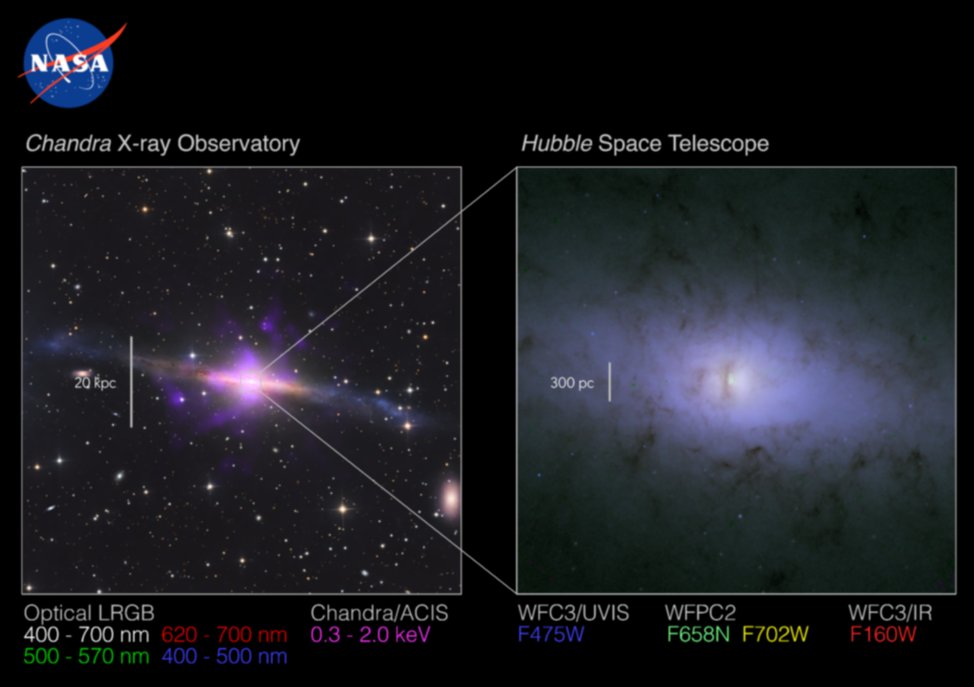
\includegraphics[trim={0 20 0 300}, clip, width=\textwidth]{FIGURES/Composition_NGC5084_poster_v6_paper.png}
\caption{Morphological structure of NGC\,5084 in X-ray, optical, and near-infrared wavelengths. \emph{Left panel:} Optical and X-ray image of 
the disk of NGC\,5084. \emph{Background:} Luminance-RGB image (Telescope: CDK17. Camera: SBIG STXL-11002M. Filter: Astrodon Gen 1 LRGB E-Series. Credit: Martin Pugh \& Brian Diaz). Field-of-view (FOV): $15\times15$ arcmin$^{2}$. \emph{Right panel:} High resolution luminance-RGB image zoom of the core of NGC\,5084 based on \emph{Hubble} Space Telescope observations. \emph{Blue:} WFC3/UVIS F475W. \emph{Green:} WFPC2 F658N. \emph{Yellow:} WFPC2 F702W. \emph{Red:} WFC3/IR F160W.  FOV: $24\times24$ arcsec$^{2}$. See the legend for color-band description and the physical scale-bars in the panels for reference.} 
\label{fig:NGC5084_poster}
\end{center}
\end{figure*}


NGC\,5084 hosts signs of past interactions which are visible in the outer regions of the galactic disk, such as a warped disk at low surface brightness intensity levels \citep{zeilinger+1990mnras246_324}, potentially related to the population of satellite galaxies within its group \citep{carignan+1997aj113_1585}. NGC\,5084 shows an unusual ratio between the $B$-band optical radius $R_{25}$ and the $K_S$-band
effective radius $R_{\rm e}$. For this galaxy, $R_{25}$ is 20 times larger than $R_e$, in contrast to $R_{25}=3.6 \times R_e$, the nominal average for spirals and S0s measured by  \citet[][]{williams+2009mnras400_1665}.  \citet{zaw+2019apj872_134} classified NGC\,5084 as an AGN according to the \citet{kewley+2001apj556_121} optical spectral line ratio criteria, based on 6dF Galaxy Survey spectra \citep{jones+2004mnras355_747,jones+2009mnras399_683}, as did \citet{irwin+2019aj158_21}, based on its radio emission (see Sec.\,\ref{subsec:data_radiopol}). In addition, NGC\,5084 is the host of a large spheroidal bulge that generates an anti-truncated surface brightness profile \citep{comeron+2012apj759_98}, a potential sign of past gravitational interactions, such as minor and major mergers \citep{younger+2007apj670_269, borlaff+2014aap570_103}.

\citet{osullivan+2017mnras472_1482} analyzed the \Chandra\ X-ray observations using the Advanced CCD Imaging Spectrometer (ACIS), concluding that the X-ray emission of NGC\,5084 is primarily generated by the central core\footnote{From \citet{osullivan+2017mnras472_1482}, about NGC\,5084: \emph{``show[ing] no evidence of a hot IGM, but does detect powerlaw emission extending $\sim100$" ($\sim$10 kpc), with a central point
source contributing the majority of the emission.}"}. No further attempt to deconvolve the Point Spread Function (PSF) or to identify the source of the emission has been published until now.  NGC\,5084 is a particularly interesting target to look for evidence of past interactions with multi-wavelength (high-resolution optical combined with wide FOV X-ray imaging) archival observations from Chandra and Hubble, in addition to millimeter (mm) and submm observations (ALMA) and radio continuum observations (EVLA). 


This project is the second publication in a series that will study the hot gas halos around galaxies using X-ray observations from the \Chandra\ X-ray observatory. The first paper \citep[][\texttt{SAUNAS I}, hereafter]{borlaff+2024apj967_169} describes the \SAUNAS\ (Selective Amplification of Ultra Noisy Astronomical Signal) pipeline to detect low surface brightness emission in \Chandra/ACIS observations. See \texttt{SAUNAS I} for the details and description of the X-ray image reduction methodology. \par 
This paper is organized as follows. The datasets and methodology pipeline is described in Sec.\,\ref{sec:methods}. The results are presented in Sec.\,\ref{sec:results}. The discussion and conclusions are presented in Sec.\,\ref{sec:DIS} and \ref{sec:CON}, respectively. All magnitudes are in the AB system \citep{oke1971apj170_193} unless otherwise noted.


\bibliography{Extragalactic}\bibliographystyle{CORE-AAS/aasjournal}


\end{document}
